\documentclass{beamer}
%
% Choose how your presentation looks.
%
% For more themes, color themes and font themes, see:
% http://deic.uab.es/~iblanes/beamer_gallery/index_by_theme.html
%
%\definecolor{title}{RGB}{75, 0, 130}
\mode<presentation>
{
  \usetheme{default}      % or try Darmstadt, Madrid, Warsaw, ...
  \usecolortheme{default} % or try albatross, beaver, crane, ...
  \usefonttheme{default}  % or try serif, structurebold, ...
  
  %\setbeamercolor{normal text}{fg=black}\usebeamercolor*{normal text}
  %\setbeamercolor{frametitle}{fg=title}\usebeamercolor*{title}
  
  \setbeamertemplate{navigation symbols}{}
  %\setbeamertemplate{caption}[numbered]
  \setbeamertemplate{caption}{\raggedright\insertcaption\par}
} 



\usepackage[russian, english]{babel}
\usepackage[utf8]{inputenc}
\usepackage[T1]{fontenc}
\usepackage[T2A]{fontenc}

\usepackage{xcolor}
\usepackage{hyperref}
% Цвета для гиперссылок
\definecolor{linkcolor}{HTML}{00008B} % цвет ссылок
\definecolor{urlcolor}{HTML}{00008B} % цвет гиперссылок

\hypersetup{pdfstartview=FitH,  linkcolor=linkcolor,urlcolor=urlcolor, colorlinks=true}


\makeatletter
\setbeamertemplate{footline}{%
  \leavevmode%
  \hbox{\begin{beamercolorbox}[wd=.3\paperwidth,ht=2.5ex,dp=1.125ex,leftskip=.3cm plus1fill,rightskip=.3cm]{}%
    \usebeamerfont{}
  \end{beamercolorbox}%
  \begin{beamercolorbox}[wd=.7\paperwidth,ht=2.5ex,dp=1.125ex,leftskip=.3cm,rightskip=.3cm plus1fil]{title in head/foot}%
    \usebeamerfont{title in head/foot}
  \end{beamercolorbox}}%
  \vskip0pt%
}
\makeatother

\title[Your Short Title]{Semiautodoc}
\author{Aleksandra Prohorova, Andrey Barekov}
\date{24 April, 2021}

\usepackage{graphicx}
\usepackage{amsmath}

\newcommand\x{\times}
\newcommand\y{\cellcolor{green!10}}
\begin{document}

\begin{frame}
  \titlepage
\end{frame}

% Uncomment these lines for an automatically generated outline.
%\begin{frame}{Outline}
%  \tableofcontents
%\end{frame}

\selectlanguage{russian}
\section{}

\section{Introduction}
\setbeamertemplate{frametitle}[default][center]
\setbeamertemplate{footline}[frame number]
\begin{frame}
{Problem}
\begin{itemize}
\item{necessity of documentation}
\item{desire to edit the documentation separately from code}
\item{opportunity of manual fix if something went wrong }
\end{itemize}

\vskip 1cm

\end{frame}

\section{Problem}
\begin{frame}
{Requirements}

\begin{itemize}
\item{automatic parsing of classes and function's names from source code}
\item{edit names that were produced as a result of parsing}
\item{add names to the current list if some of them were missed and delete names that seem unimportant, add despription for each element to get most relevant documentation}
\item{get readable markdown file from tree structure of classes and functions}
\end{itemize}

%GUI application aiming to simplify writing of documentation for source
%code: parsing gives logically significant units (classes and functions), formed
%in a tree structure, that can be interactively changed, filled and eventually %converted to markdown file.

\hskip 2.1cm

\end{frame}



\section{Model}
\begin{frame}
{Project structure}
\vskip 0.1cm

\begin{itemize}
\item{static library for parsing}
\item{unit and functional tests for static library}
\item{GUI}
\end{itemize}

\end{frame}

\begin{frame}
{Example}{Results of parsing}
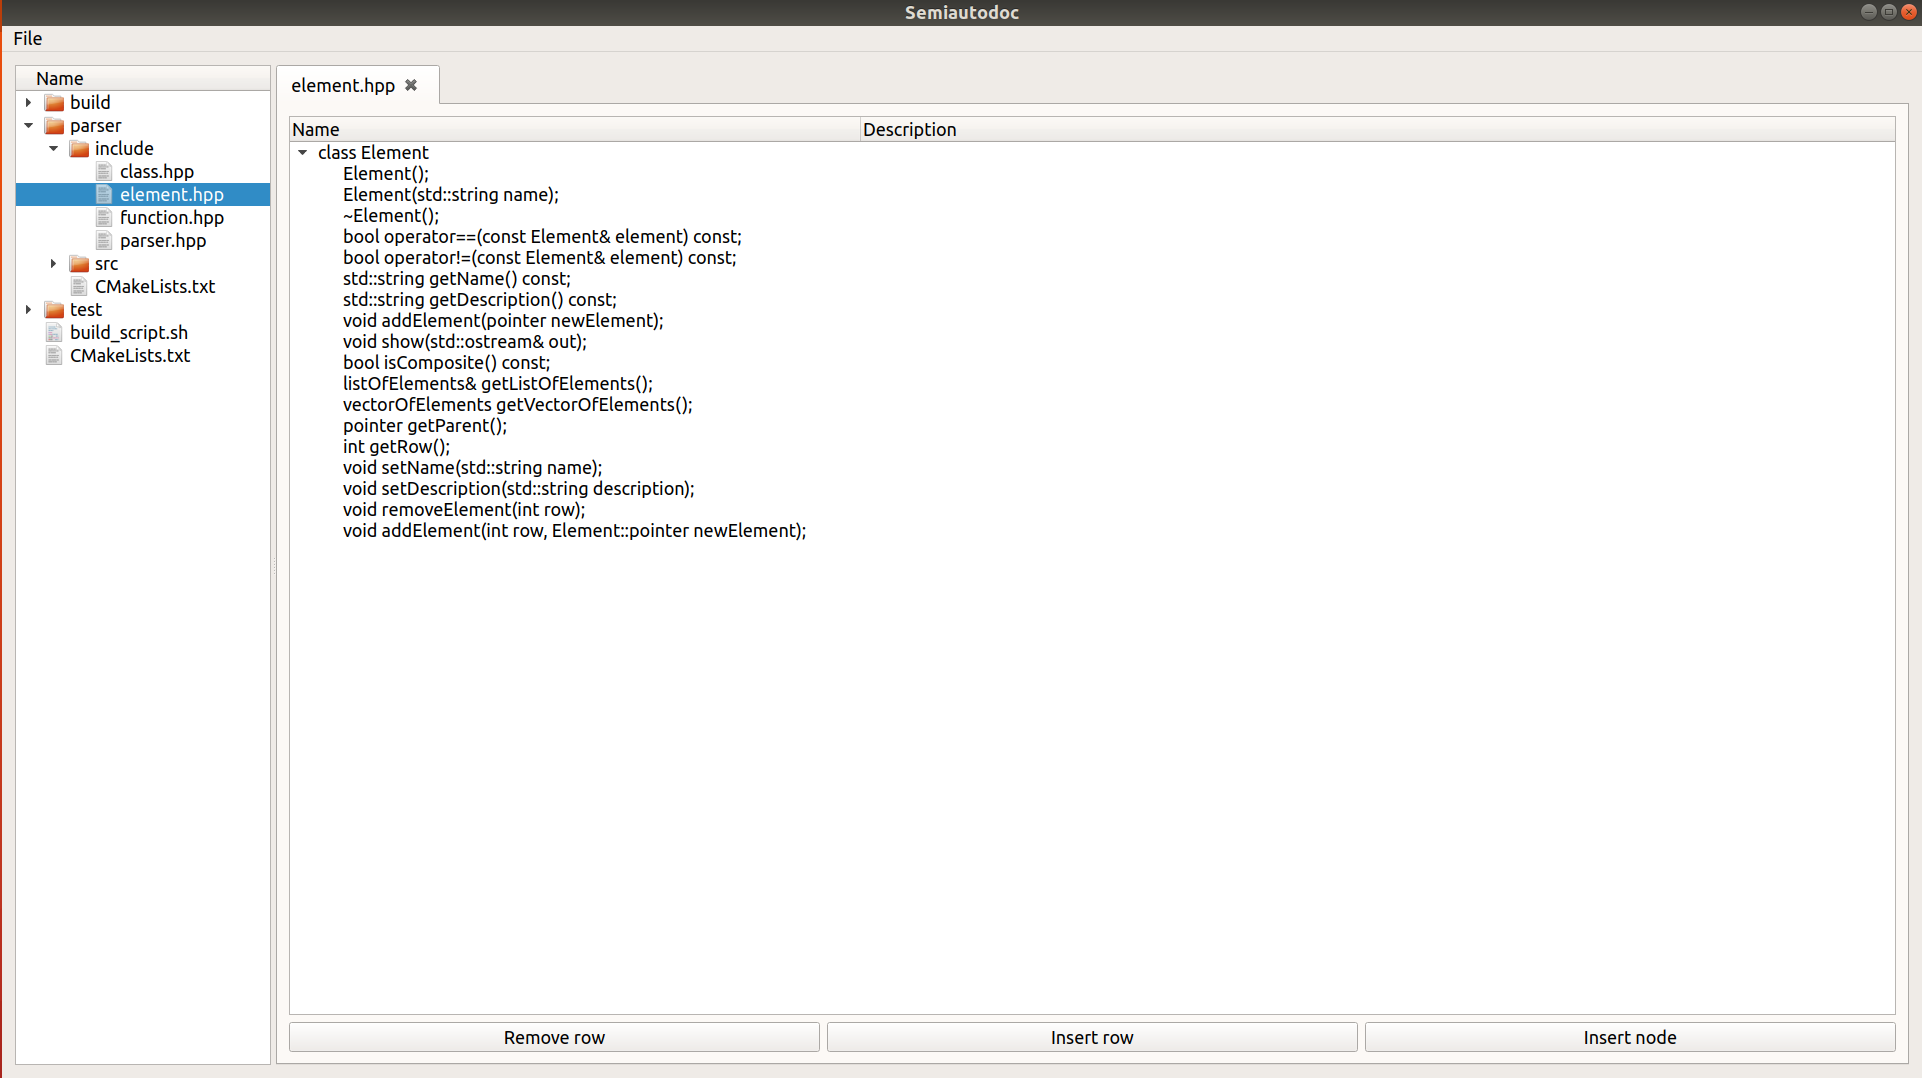
\includegraphics[scale = 0.28]{semiautodoc-example.png}
%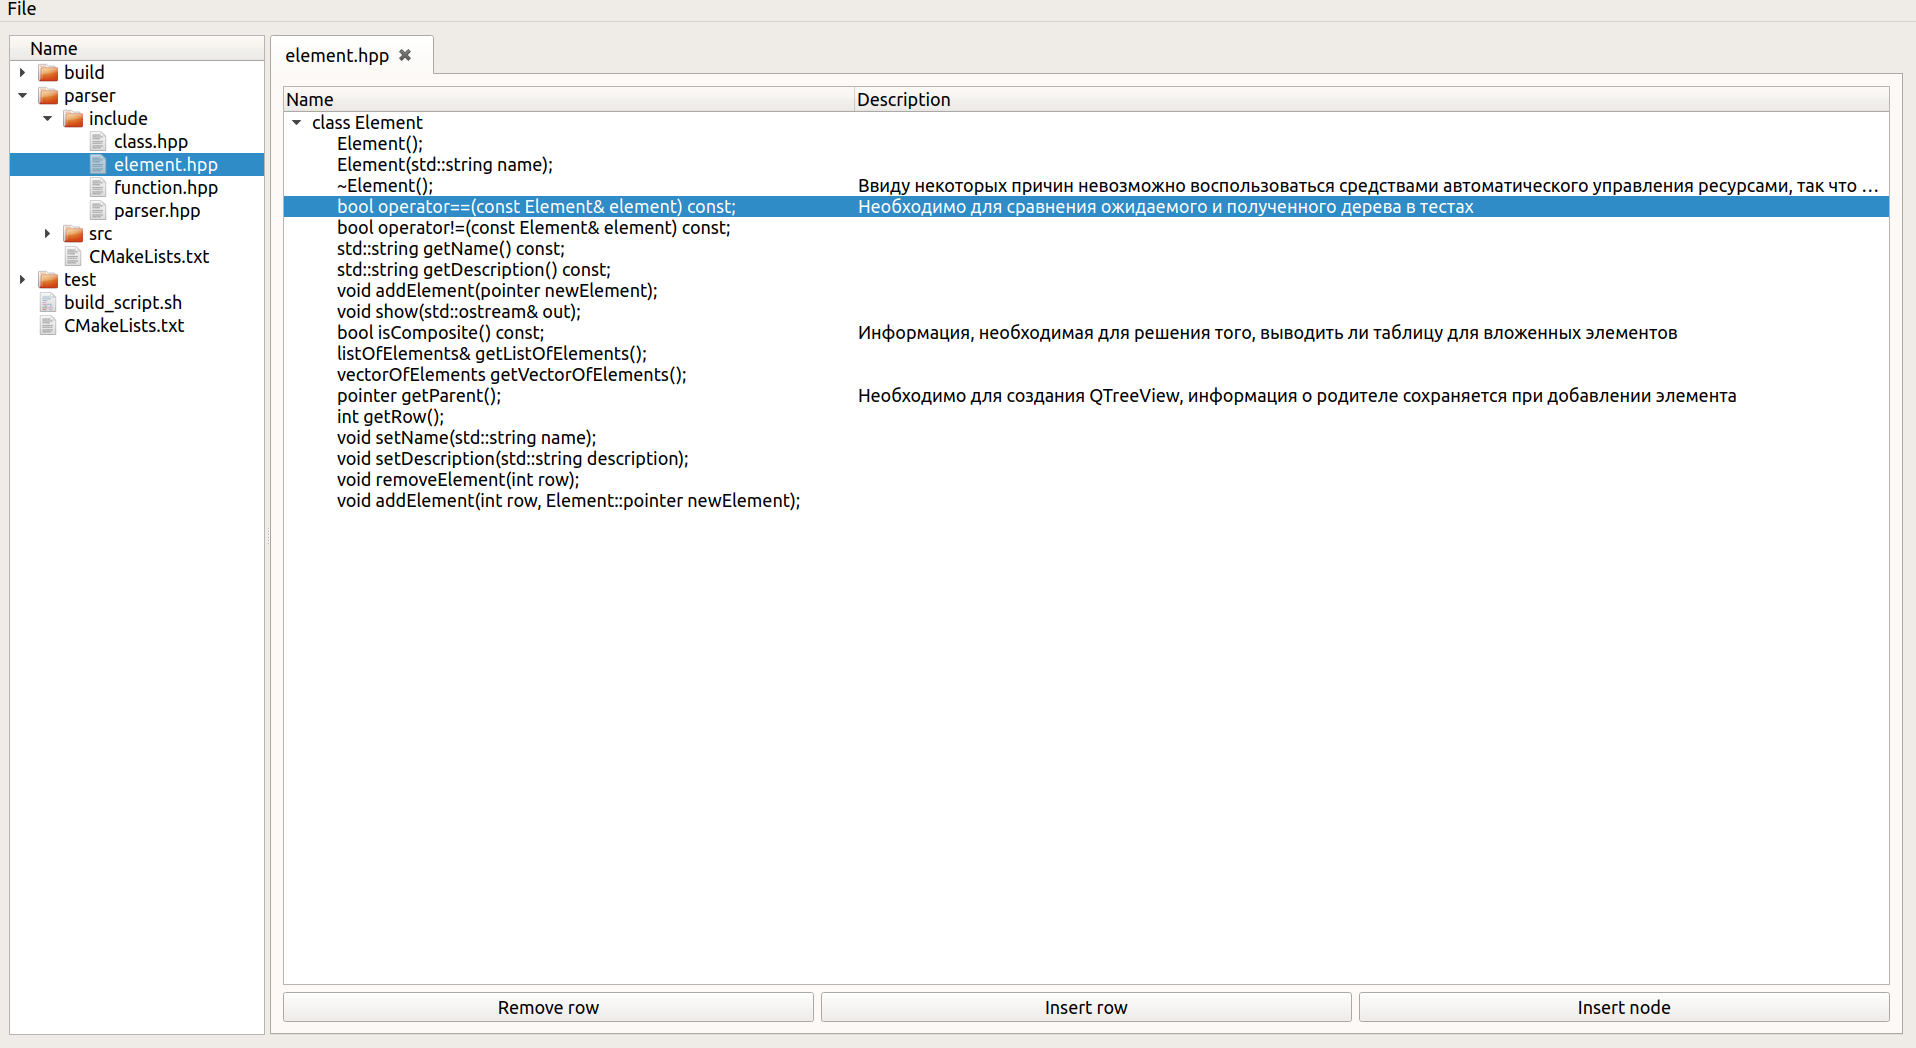
\includegraphics[scale = 0.45]{edit.png}\\\\

%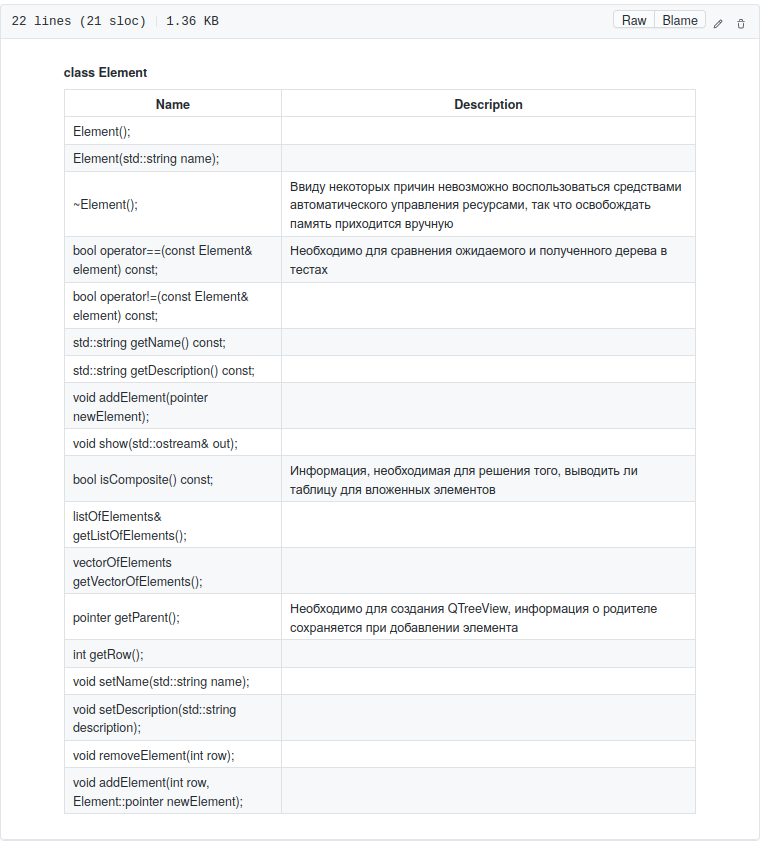
\includegraphics[scale = 0.75]{markdown.png}\\\\

\end{frame}

\begin{frame}
{Example}{Edit results of parsing}
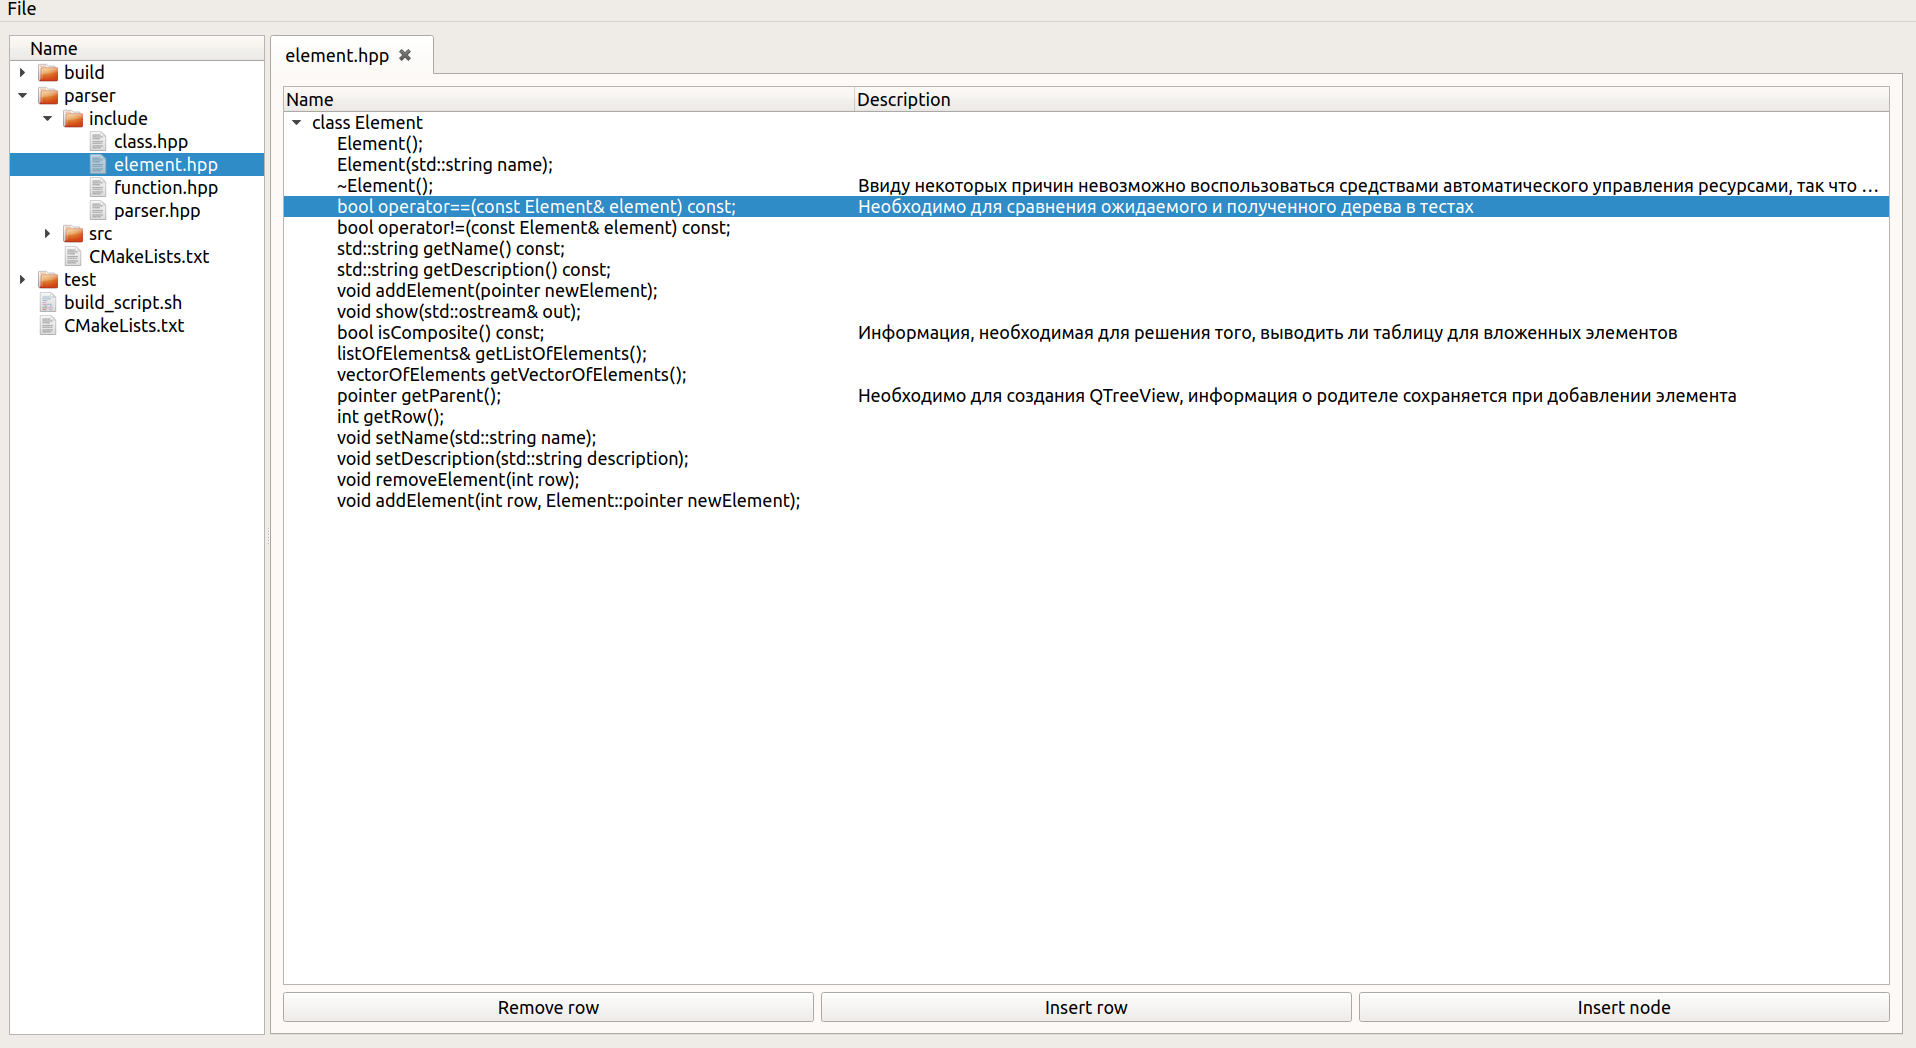
\includegraphics[scale = 0.28]{edit.png}

%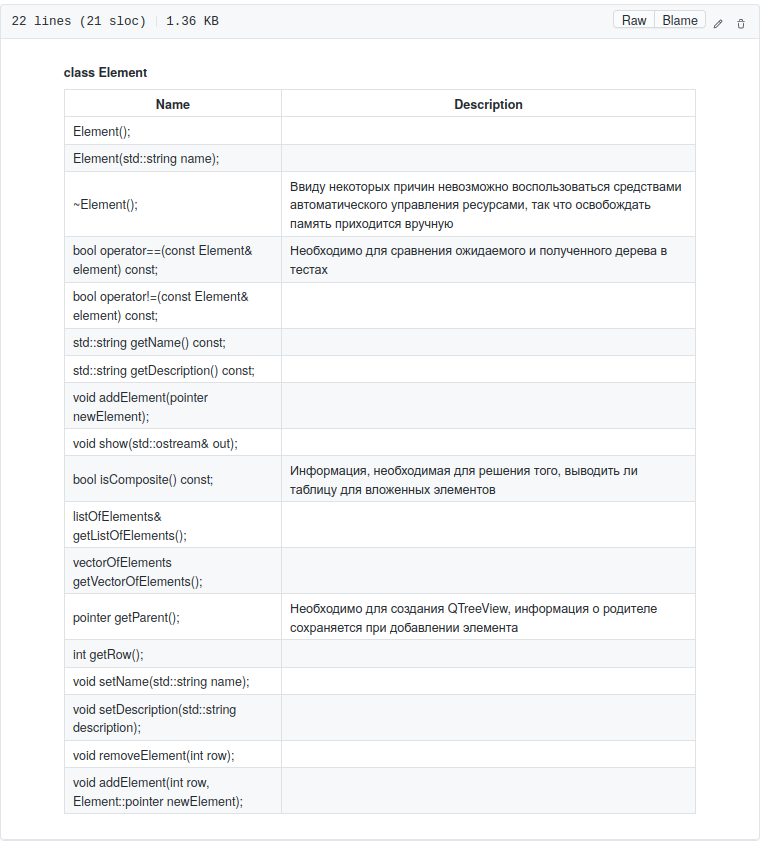
\includegraphics[scale = 0.75]{markdown.png}\\\\

\end{frame}

\begin{frame}
{Example}{Markdown file}

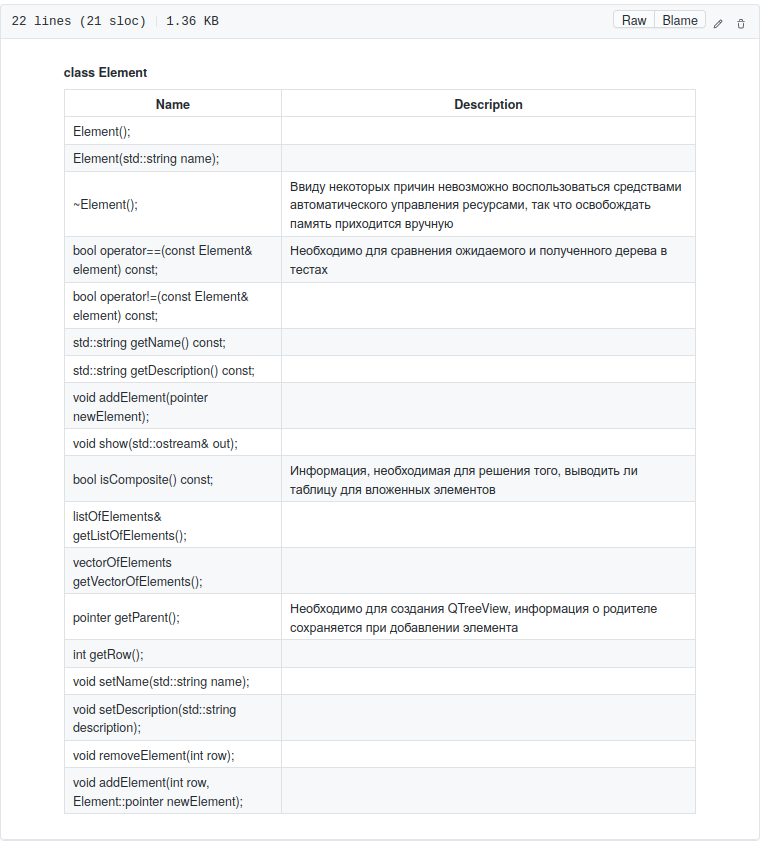
\includegraphics[scale = 0.4]{markdown.png}

\end{frame}


\begin{frame}
{Source code}
\href{https://github.com/aleksandraprohorova/semiautodoc}{\textbf{https://github.com/aleksandraprohorova/semiautodoc}}\\
\end{frame}



\end{document}